\RequirePackage{currfile}
\documentclass[12pt]{beamer}
\usepackage[utf8]{inputenc}
\usepackage[spanish]{babel}
\usepackage{standalone}
\usepackage{color}
\usepackage{siunitx}
\usepackage{hyperref}
\usepackage[outdir=./]{epstopdf}
%\hypersetup{colorlinks,linkcolor=,urlcolor=blue}
%\hypersetup{colorlinks,urlcolor=blue}
\usepackage{xcolor,soul}
\usepackage{etoolbox}
\usepackage{amsmath}
\usepackage{amsthm}
\usepackage{mathtools}
\usepackage{tcolorbox}
\usepackage{physics}
\usepackage{multicol}
\usepackage{bookmark}
\usepackage{longtable}
\usepackage{listings}
\usepackage{cancel}
\usepackage{wrapfig}
\usepackage{empheq}
\usepackage{graphicx}
\usepackage{tikz}
\usetikzlibrary{calc, patterns, matrix, backgrounds, decorations,shapes, arrows.meta}
\usepackage[autostyle,spanish=mexican]{csquotes}
\usepackage[os=win]{menukeys}
\usepackage{pifont}
\usepackage{pbox}
\usepackage{bm}
\usepackage{caption}
\captionsetup{font=scriptsize,labelfont=scriptsize}
%\usepackage[sfdefault]{roboto}  %% Option 'sfdefault' only if the base font of the document is to be sans serif

%Sección de definición de colores
\definecolor{ao}{rgb}{0.0, 0.5, 0.0}
\definecolor{bisque}{rgb}{1.0, 0.89, 0.77}
\definecolor{amber}{rgb}{1.0, 0.75, 0.0}
\definecolor{armygreen}{rgb}{0.29, 0.33, 0.13}
\definecolor{alizarin}{rgb}{0.82, 0.1, 0.26}
\definecolor{cadetblue}{rgb}{0.37, 0.62, 0.63}
\definecolor{deepblue}{rgb}{0,0,0.5}
\definecolor{brown}{rgb}{0.59, 0.29, 0.0}
\definecolor{OliveGreen}{rgb}{0,0.25,0}
\definecolor{mycolor}{rgb}{0.122, 0.435, 0.698}

\newcommand*{\boxcolor}{orange}
\makeatletter
\newcommand{\boxedcolor}[1]{\textcolor{\boxcolor}{%
\tikz[baseline={([yshift=-1ex]current bounding box.center)}] \node [rectangle, minimum width=1ex, thick, rounded corners,draw] {\normalcolor\m@th$\displaystyle#1$};}}
 \makeatother

\newtcbox{\mybox}{on line,
  colframe=mycolor,colback=mycolor!10!white,
  boxrule=0.5pt,arc=4pt,boxsep=0pt,left=6pt,right=6pt,top=6pt,bottom=6pt}

\usefonttheme[onlymath]{serif}
%Sección de definición de nuevos comandos

\newcommand*{\TitleParbox}[1]{\parbox[c]{1.75cm}{\raggedright #1}}%
\newcommand{\python}{\texttt{python}}
\newcommand{\textoazul}[1]{\textcolor{blue}{#1}}
\newcommand{\azulfuerte}[1]{\textcolor{blue}{\textbf{#1}}}
\newcommand{\funcionazul}[1]{\textcolor{blue}{\textbf{\texttt{#1}}}}
\newcommand{\ptilde}[1]{\ensuremath{{#1}^{\prime}}}
\newcommand{\stilde}[1]{\ensuremath{{#1}^{\prime \prime}}}
\newcommand{\ttilde}[1]{\ensuremath{{#1}^{\prime \prime \prime}}}
\newcommand{\ntilde}[2]{\ensuremath{{#1}^{(#2)}}}
\renewcommand{\arraystretch}{1.5}

\newcounter{saveenumi}
\newcommand{\seti}{\setcounter{saveenumi}{\value{enumi}}}
\newcommand{\conti}{\setcounter{enumi}{\value{saveenumi}}}
\renewcommand{\rmdefault}{cmr}% cmr = Computer Modern Roman

\linespread{1.5}

\usefonttheme{professionalfonts}
%\usefonttheme{serif}
\DeclareGraphicsExtensions{.pdf,.png,.jpg}


%Sección para el tema de beamer, con el theme, usercolortheme y sección de footers
\mode<presentation>
{
  \usetheme{Warsaw}
  
  %\useoutertheme{infolines}
  \useoutertheme{default}
  \usecolortheme{crane}
  \setbeamercovered{invisible}
  % or whatever (possibly just delete it)
  \setbeamertemplate{section in toc}[sections numbered]
  \setbeamertemplate{subsection in toc}[subsections numbered]
  \setbeamertemplate{subsection in toc}{\leavevmode\leftskip=3.2em\rlap{\hskip-2em\inserttocsectionnumber.\inserttocsubsectionnumber}\inserttocsubsection\par}
  % \setbeamercolor{section in toc}{fg=blue}
  % \setbeamercolor{subsection in toc}{fg=blue}
  % \setbeamercolor{frametitle}{fg=blue}
  \setbeamertemplate{caption}[numbered]

  \setbeamertemplate{footline}
  \beamertemplatenavigationsymbolsempty
  \setbeamertemplate{headline}{}
}

\makeatletter
\setbeamercolor{section in foot}{bg=brown!75, fg=white}
\setbeamercolor{subsection in foot}{bg=cadetblue}
\setbeamertemplate{footline}
{
  \leavevmode%
  \hbox{%
  \begin{beamercolorbox}[wd=.333333\paperwidth,ht=2.25ex,dp=1ex,center]{section in foot}%
    \usebeamerfont{section in foot} \insertsection
  \end{beamercolorbox}}%
  \begin{beamercolorbox}[wd=.333333\paperwidth,ht=2.25ex,dp=1ex,center]{subsection in foot}%
    \usebeamerfont{subsection in foot}  \insertsubsection
  \end{beamercolorbox}%
  \begin{beamercolorbox}[wd=.333333\paperwidth,ht=2.25ex,dp=1ex,right]{date in head/foot}%
    \usebeamerfont{date in head/foot} \insertshortdate{} \hspace*{2em}
    \insertframenumber{} / \inserttotalframenumber \hspace*{2ex} 
  \end{beamercolorbox}}%
  \vskip0pt%
\makeatother  

\makeatletter
\patchcmd{\beamer@sectionintoc}
  {\vfill}
  {\vskip\itemsep}
  {}
  {}
\makeatother


\title{\large{Gram-Schmidt y Completez}}
\subtitle{Ejercicios}
\author{M. en C. Gustavo Contreras Mayén}
\date{}
\institute{Facultad de Ciencias - UNAM}
\titlegraphic{
\includegraphics[width=1.75cm]{../Imagenes/escudo-facultad-ciencias}\hspace*{4.75cm}~%
   
\includegraphics[width=1.75cm]{../Imagenes/escudo-unam}
}
\setbeamertemplate{navigation symbols}{}
\begin{document}
\maketitle
\fontsize{14}{14}\selectfont
\spanishdecimal{.}
\section*{Contenido}
\frame[allowframebreaks]{\tableofcontents[currentsection, hideallsubsections]}
\section{Gram-Schmidt}
\frame{\tableofcontents[currentsection, hideothersubsections]}
\subsection{Ejercicio Ortogonalización}
\begin{frame}
\frametitle{Ejercicio}
Usando el método de ortogonalización de Gram-Schmidt construye los primeros tres polinomios de Hermite, usando:
\begin{align*}
&u_{n}(x) = x^{n}, \hspace{2.5cm} n = 0, 1, 2, \ldots, \\[0.5cm]
&-\infty < x < \infty, \hspace{1cm} \omega(x) = e^{-x^{2}}
\end{align*}
\end{frame}
\begin{frame}
\frametitle{Ejercicio}
Para este ejercicio la normalización del conjunto de polinomios es:
\begin{align*}
\int_{-\infty}^{\infty} H_{m} (x) \, H_{n} (x) \, \omega (x) \dd{x} = \delta_{mn} \, 2^{m} \, m! \, \pi^{1/2}
\end{align*}
\end{frame}
\begin{frame}
\frametitle{Ortogonalización de Gram-Schmidt}
De acuerdo a las notas de trabajo, la ortogonalización de Gram-Schmidt requiere desarrollar la expresión de las $\psi_{n} (x)$, que son funciones linealmente independientes, ortogonales pero no normalizadas:
\begin{align*}
\psi_{i} (x) = u_{i} + a_{i,0} \, \varphi_{0} + a_{i,1} \, \varphi_{1} + \ldots + a_{i,i-1} \, \varphi_{i-1} 
\end{align*}
\end{frame}
\begin{frame}
\frametitle{Ortogonalización de Gram-Schmidt}
Los coeficientes $a_{i, j}$ están dados por
\begin{align*}
a_{i,j} = - \dfrac{\displaystyle \int u_{i}(x) \, \varphi_{j} (x) \, \omega (x) \dd{x}}{N_{j}^{2}}
\end{align*}
además:
\begin{align*}
\int_{a}^{b} \left[ \varphi_{j} (x) \right]^{2} \, \omega (x) \dd{x} = N_{j}^{2}
\end{align*}
\end{frame}
\begin{frame}
\frametitle{Ortogonalización de Gram-Schmidt}
Las funciones $\varphi_{i}(x)$ son linealmente independientes, ortogonales y ya normalizadas, el término $N_{i}$ lo tomamos de la normalización del conjunto de polinomios:
\begin{align*}
\varphi_{i} (x) = N_{i} \, \dfrac{\psi_{i}}{\left[ \displaystyle \int \psi_{i}^{2} (x) \, \omega (x) \dd{x} \right]^{1/2}}
\end{align*}
\end{frame}
\subsection{Desarrollo}
\begin{frame}
\frametitle{Para $n = 0$}
Comenzamos con el índice $n = 0$, por lo que:
\begin{eqnarray*}
\psi_{0}(x) = u_{0} (x) = \pause x^{0} =  1
\end{eqnarray*}
\pause
Al ser el primer término, procedemos a normalizar:
\begin{align*}
\varphi_{0} (x) = N_{0} \, \dfrac{\psi_{0}(x)}{\left[ \displaystyle \int \psi_{0}^{2} (x) \, \omega (x) \dd{x} \right]^{1/2}} =
\end{align*}
\end{frame}
\begin{frame}
\frametitle{Para $n = 0$}
Sustituyendo:
\begin{eqnarray*}
N_{0}^{2} &=& 2^{0} \, 0! \, \pi^{1/2} = \pi^{1/2} \\[0.5em] \pause
N_{0} &=& \left[ \pi^{1/2} \right]^{1/2} = \pi^{1/4}
\end{eqnarray*}
\pause
Entonces\footnote<3->{En los ejercicios se deberán de explicitar la solución de las integrales.}:
\begin{align*}
\varphi_{0} (x) = \pi^{1/4} \, \dfrac{1}{\left[ \displaystyle \int e^{-x^{2}} \dd{x} \right]^{1/2}} =
\end{align*}
\end{frame}
\begin{frame}
\frametitle{Obteniendo $\varphi_{0} (x)$}
Por lo que
\begin{eqnarray*}
\varphi_{0} (x) &=& \pi^{1/4} \, \dfrac{1}{\left[ \pi^{1/2} \right]^{1/2}} = \\[1em] \pause
&=& \dfrac{\pi^{1/4}}{\pi^{1/4}} =
\end{eqnarray*}
\pause
\begin{align*}
\setlength{\fboxsep}{3\fboxsep}\boxed{
\varphi_{0} (x) = 1}
\end{align*}
\end{frame}
\begin{frame}
\frametitle{Con $n = 1$}
Debemos de obtener:
\begin{align*}
\psi_{1} (x) = u_{1} + a_{1,0} \, \varphi_{0}
\end{align*}
\pause
donde:
\begin{eqnarray*}
u_{1} &=& x^{1} = x \\[0.5em] \pause
a_{1,0} &=& - \dfrac{\displaystyle \int_{-\infty}^{\infty} u_{1}(x) \, \varphi_{0} (x) \, \omega (x) \dd{x}}{N_{0}^{2}}
\end{eqnarray*}
\end{frame}
\begin{frame}
\frametitle{Con $n = 1$}
Calculamos $N_{0}^{2}$, así:
\pause
\begin{align*}
N_{0}^{2} = \pi^{1/2}
\end{align*}
\pause
Por tanto
\begin{eqnarray*}
a_{1,0} &=& - \dfrac{1}{\pi^{1/2}} \, \int_{-\infty}^{\infty} x \, e^{-x^{2}} \dd{x} = \pause 0
\end{eqnarray*}
\pause
Así llegamos a:
\begin{align*}
\psi_{1} (x) = x
\end{align*}
Procedamos a normalizar
\end{frame}
\begin{frame}
\frametitle{Con $n = 1$}
Normalizando:
\begin{align*}
\varphi_{1}(x) = N_{1} \, \dfrac{\psi_{1}}{\left[ \displaystyle \int \psi_{1}^{2} \, \omega \dd{x} \right]^{1/2}}
\end{align*}
\pause
Calculamos ahora $N_{1}$, por lo que
\begin{align*}
N_{1}^{2} &= 2 \, \pi^{1/2} \\[0.5em]
N_{1} &= \sqrt{2} \, \pi^{1/4}
\end{align*}
\end{frame}
\begin{frame}
\frametitle{Con $n = 1$}
Tendremos:
\fontsize{12}{12}\selectfont
\begin{eqnarray*}
\varphi_{1}(x) &=& \dfrac{x \, \sqrt{2} \, \pi^{1/4}}{\left[ \displaystyle \int x^{2} \, e^{-x^{2}} \dd{x} \right]^{1/2}} = \\[0.5em] \pause
&=& \dfrac{x \, \sqrt{2} \, \pi^{1/4}}{ \left[ \dfrac{\sqrt{\pi}}{2} \right]^{1/2}} = \pause \dfrac{x \, \sqrt{2} \, \sqrt{2} \, \pi^{1/4}}{\pi^{1/4}} =
\end{eqnarray*}
\pause
\begin{align*}
\setlength{\fboxsep}{3\fboxsep}\boxed{
\varphi_{1}(x) = 2 \, x }
\end{align*}
\end{frame}
\begin{frame}
\frametitle{Con $n = 2$}
El desarrollo a resolver es:
\begin{align*}
\psi_{2} (x) = u_{2} + a_{2,0} \, \varphi_{0} + a_{2,1} \, \varphi_{1}
\end{align*}
\pause
Donde:
\fontsize{12}{12}\selectfont
\begin{align*}
u_{2}(x) &= x^{2} \\[0.5em]
a_{2,0} &= - \dfrac{\displaystyle \int_{-\infty}^{\infty} u_{2}(x) \, \varphi_{0}(x) \, \omega (x) \dd{x}}{N_{0}^{2}} \\[0.5em]
a_{2,1} &= - \dfrac{\displaystyle \int_{-\infty}^{\infty} u_{2}(x) \, \varphi_{1}(x) \, \omega (x) \dd{x}}{N_{1}^{2}}
\end{align*}
\end{frame}
\begin{frame}
\frametitle{Con $n =  2$}
Se tiene que:
\begin{align*}
N_{0}^{2} &= \pi^{1/2} \\[0.5em]
N_{1}^{2} &= 2 \, \pi^{1/2}
\end{align*}
\pause
Entonces tendremos que:
\begin{align*}
a_{2,0} &= - \dfrac{1}{\pi^{1/2}} \int_{-\infty}^{\infty} x^{2} \, e^{-x^{2}} \dd{x} \\[0.5em]
a_{2,1} &= - \dfrac{1}{2 \, \pi^{1/2}} \int_{-\infty}^{\infty} 2\, x^{3} \, e^{-x^{2}} \dd{x}
\end{align*}
\end{frame}
\begin{frame}
\frametitle{Con $n =  2$}
Resolviendo las integrales llegamos a:
\begin{align*}
a_{2,0} &= - \dfrac{1}{2} \\[0.5em]
a_{2,1} &= 0
\end{align*}
La segunda integral se anula.
\\
\pause
Por lo que:
\begin{align*}
\psi_{2} (x) = x^{2} - \dfrac{1}{2}
\end{align*}
Pasamos a normalizar.
\end{frame}
\begin{frame}
\frametitle{Obteniendo $\varphi_{2}(x)$}
Sabemos que normalizando:
\begin{align*}
\varphi_{2} (x) = N_{2} \, \dfrac{ \psi_{2}}{\left[ \displaystyle \int \psi_{2}^{2} \, \omega \dd{x} \right]^{1/2}}
\end{align*}
\pause
Con
\begin{align*}
N_{2} = 2 \, \sqrt{2} \, \pi^{1/4}
\end{align*}
\end{frame}
\begin{frame}
\frametitle{Obteniendo $\varphi_{2}(x)$}
Sustituyendo:
\begin{align*}
\varphi_{2} (x) = \dfrac{\bigg(2 \, \sqrt{2} \, \pi^{1/4} \bigg) \left(x^{2} - \dfrac{1}{2} \right)}{\left[ \displaystyle \int \left(x^{2} - \dfrac{1}{2} \right)^{2} \, e^{-x^{2}} \dd{x} \right]^{1/2}}
\end{align*}
\pause
Se desarrolla el binomio del integrando en el denominador, de tal manera que:
\end{frame}
\begin{frame}
\frametitle{Obteniendo $\varphi_{2}(x)$}
Resolviendo el álgebra:
\begin{eqnarray*}
\varphi_{2} (x) &=& \dfrac{\bigg(2 \, \sqrt{2} \, \pi^{1/4} \bigg) \left(x^{2} - \dfrac{1}{2} \right)}{\left[ \dfrac{\sqrt{\pi}}{2}\right]^{1/2}} = \\[0.5em] \pause
&=& \dfrac{\bigg(2 \, \sqrt{2} \, \sqrt{2} \, \pi^{1/4} \bigg) \left(x^{2} - \dfrac{1}{2} \right)}{\pi^{1/4}} =
\end{eqnarray*}
\end{frame}
\begin{frame}
\frametitle{Obteniendo $\varphi_{2}(x)$}
Concluimos que:
\begin{align*}
\setlength{\fboxsep}{3\fboxsep}\boxed{
\varphi_{2} (x) = 4 \, x^{2} - 2 }
\end{align*}
\end{frame}
\begin{frame}
\frametitle{Solución}
Entonces los tres primeros polinomios que se obtienen con el método de ortogonalización de Gram-Schmidt son:
\begin{align*}
\varphi_{0} (x) &= 1 \\[0.5em]
\varphi_{1} (x) &= 2 \, x \\[0.5em]
\varphi_{2} (x) &= 4 \, x^{2} - 2
\end{align*}
Que corresponden a los polinomios de Hermite: $H_{0}(x)$, $H_{1}(x)$ y $H_{2}(x)$.
\end{frame}
\begin{frame}
\frametitle{Gráfica de los $H{n}(x)$}
\begin{figure}[H]
   \centering
   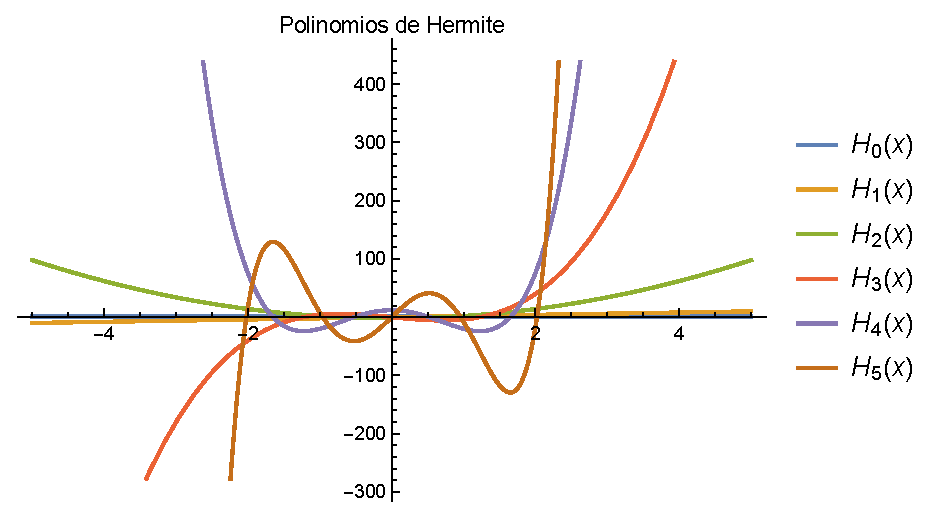
\includegraphics[scale=0.7]{Imagenes/Plot_Hermite.eps}
   \caption{Gráfica de los primeros polinomios de Hermite $H_{n}(x)$.}
\end{figure}
\end{frame}
\end{document}